% Provenance (never printed): see sources/outline_sources.md (Year 3: refraction and
% reflection seismic methods; CMP acquisition, NMO, stacking, Dix; migration in
% principle; seismic stratigraphy). Brief: sources/book5/BRIEFS.md, ch. 2. Curves from
% figdata/bachelor-3/seismic_model.py, refraction_dip.py, synthetic_seismogram.py,
% cmp_nmo.py (the Varden column, region.py); exercise and problem values in the
% Book 5 scratch calculator calc/ch02.py.
\chapter{Exploration Seismology}\label{ch:b3:exploration-seismology}

A survey vessel steams slowly along a straight line at sea, towing an array of
air guns a few metres below the surface and, behind it, cables several
kilometres long studded with hydrophones. In one survey described to the
regulator, the array held \num{5240} cubic inches of compressed air, fired every
\qty{8}{s} from \qty{12}{m} below the surface, and the narrow-azimuth streamers
behind such vessels record offsets of 8 to \qty{10}{km}.
% ledger: noaa5:wg-survey
Each shot sends a pulse of sound into the sea floor, and every rock interface
below returns a faint echo. Weeks of processing later, a geologist scrolls
through a cross-section in which buried river channels, tilted fault blocks and
the onlapping fill of an old basin appear as if the ground had been cut open.
The Earth-scale seismology of the previous chapter used the waves of
earthquakes; exploration seismology makes its own, with sources whose time and
place are known exactly, and records them on thousands of channels. This
chapter follows the echoes from the shot to the section: refraction surveys,
the reflection of a wavelet by a layered column, the common-midpoint method
that turns repeated echoes into velocities and a clean image, migration, which
puts the reflectors back where they belong, and the reading of the section as
stratigraphy.

\begin{recall}
At a boundary between two media of acoustic impedances $Z_1 = \rho_1v_1$ and
$Z_2 = \rho_2v_2$, a plane wave at normal incidence is reflected with the
amplitude coefficient $R = (Z_2 - Z_1)/(Z_2 + Z_1)$ (the physics books' Year 2
volume, on waves at interfaces). The head wave, the intercept time and the
crossover distance of a refraction profile over flat layers were met in the
Year 1 volume, in its chapter on the layered Earth; borehole logs in Book 2
(grade 11). The convolution $(f*g)(t) = \int f(\tau)g(t - \tau)\,\mathrm d\tau$
and the Fourier transform are the mathematics books'. The \omterm{def:b3:seismology-imaging:ray-parameter}{ray parameter} and the
linear \omterm{def:b3:seismology-imaging:inverse}{inverse problem} are those of \cref{ch:b3:seismology-imaging}.
\end{recall}

\section{Refraction surveys}

\begin{definition}[Seismic refraction and reflection surveys]\label{def:b3:exploration-seismology:surveys}
A \emph{seismic refraction survey}\index{seismic refraction survey} records, along
a line of receivers, the first arrivals from a controlled source, and uses the
head waves that travel along the top of faster layers to find their speeds and
depths. A \emph{seismic reflection survey}\index{seismic reflection survey}
records the whole wave train, at offsets mostly smaller than the depths of
interest, and uses the waves reflected at near-normal incidence by the
interfaces to image the layering.
\end{definition}

Over flat layers a head wave arrives at $t = x/v_2 + t_i$, a straight line
whose slope gives the speed $v_2$ of the refractor and whose intercept $t_i$
gives its depth. A dipping refractor tilts the line: the head wave shot
down-dip arrives later and later, as the refractor goes deeper, and seems slow;
shot up-dip it seems fast. Shooting both ways along the same line, a reversed
profile, separates the speed from the dip.

\begin{theorem}[Refraction on a dipping interface]\label{thm:b3:exploration-seismology:dipping}
A layer of speed $v_1$ overlies a plane refractor of speed $v_2 > v_1$ dipping
at the angle $\theta$ along the profile; $i_c = \arcsin(v_1/v_2)$, and $h$ is the
perpendicular depth of the refractor under the shot. Beyond the critical
distance, the head wave arrives at
\begin{align*}
  t &= \frac{x\sin(i_c + \theta)}{v_1} + \frac{2h\cos i_c}{v_1}
  &&\text{shooting down-dip},\\
  t &= \frac{x\sin(i_c - \theta)}{v_1} + \frac{2h\cos i_c}{v_1}
  &&\text{shooting up-dip}.
\end{align*}
The apparent speeds $v_d = v_1/\sin(i_c + \theta)$ and
$v_u = v_1/\sin(i_c - \theta)$ of a reversed profile give
\[
  i_c = \tfrac12\left[\arcsin\frac{v_1}{v_d} + \arcsin\frac{v_1}{v_u}\right],\qquad
  \theta = \tfrac12\left[\arcsin\frac{v_1}{v_d} - \arcsin\frac{v_1}{v_u}\right],
  \qquad v_2 = \frac{v_1}{\sin i_c} .
\]
\end{theorem}

\begin{proof}
Rotate the frame so that the refractor is horizontal; the surface then dips at
$\theta$, and shooting down-dip the perpendicular depth under a receiver at
offset $x$ is $h + x\sin\theta$, its projection on the refractor
$x\cos\theta$. The head-wave path goes down at the critical angle $i_c$ to the
normal, along the refractor at $v_2$, and up at $i_c$. Its time is
\[
  t = \frac{h}{v_1\cos i_c} + \frac{x\cos\theta - h\tan i_c - (h + x\sin\theta)\tan i_c}{v_2}
  + \frac{h + x\sin\theta}{v_1\cos i_c}.
\]
With $1/v_2 = \sin i_c/v_1$ and $1/\cos i_c - \sin i_c\tan i_c = \cos i_c$,
the terms in $h$ give $2h\cos i_c/v_1$ and those in $x$ give
$x(\sin i_c\cos\theta + \cos i_c\sin\theta)/v_1 = x\sin(i_c + \theta)/v_1$.
Up-dip, $\theta$ changes sign. The last formulas invert the two apparent
speeds.
\end{proof}

The two branches of a reversed profile must give the same time between the two
shot points, whichever end fired: the \emph{reciprocal time}, a check on the
picking. Two situations defeat the method. A layer slower than the one above it
(a velocity inversion) refracts no head wave and is invisible: its rocks are
counted in the layer above, and every depth below is overestimated. A layer
faster than the one above but too thin may never give a first arrival, because
the head wave of the deeper, faster layer overtakes it: a hidden layer. A
reflection survey sees both.

\begin{omfigure}
\begin{tikzpicture}
\begin{axis}[omrecord, width=0.82\linewidth, height=0.46\linewidth,
  xmin=0, xmax=1200, ymin=0, ymax=660,
  xlabel={position along the spread, from shot W (\unit{m})},
  ylabel={time (\unit{ms})}, legend pos=north west, legend cell align=left,
  legend style={font=\scriptsize}]
\addplot[gray, thick, densely dashed] table[x=x, y=tdir] {figdata/out/bachelor-3-refraction_dip-west.dat};
\addlegendentry{direct waves ($v_1$)}
\addplot[blue!70!black, thick] table[x=x, y=thead] {figdata/out/bachelor-3-refraction_dip-west.dat};
\addlegendentry{head wave from W, shot up-dip}
\addplot[red!70!black, thick] table[x expr=1200-\thisrow{x}, y=thead] {figdata/out/bachelor-3-refraction_dip-east.dat};
\addlegendentry{head wave from E, shot down-dip}
\addplot[gray, thick, densely dashed, forget plot] table[x expr=1200-\thisrow{x}, y=tdir] {figdata/out/bachelor-3-refraction_dip-east.dat};
\addplot[only marks, mark=*, mark size=1.5pt] coordinates {(1200,486.13) (0,486.13)};
\node[font=\scriptsize, anchor=south east] at (axis cs:1190,530) {reciprocal time};
\end{axis}
\end{tikzpicture}

\par\smallskip{\small A reversed refraction profile on the west limb of the
Varden anticline (computed; problem, Part I). The refractor, the top of the
limestone, rises from W to E at \ang{10.8} under a \qty{1200}{m} spread; the
chalk and shale above are lumped into one layer of \qty{2.40}{km.s^{-1}}. The
head wave shot up-dip from W appears fast (\qty{6.57}{km.s^{-1}}), the one shot
down-dip from E slow (\qty{3.52}{km.s^{-1}}); both take \qty{486.1}{ms} to cross
the whole spread. The head waves overtake the direct waves only near the far
end: the refractor is deep for so short a spread.}
\label{fig:b3:exploration-seismology:refraction}
\end{omfigure}

\section{Reflection at normal incidence}

\begin{definition}[Seismic wavelet, Ricker wavelet]\label{def:b3:exploration-seismology:wavelet}
A \emph{seismic wavelet}\index{seismic wavelet} is the short pulse, a few tens
of milliseconds long, that a source and the recording system send through the
ground; each reflector returns a scaled copy of it. The \emph{Ricker
wavelet}\index{Ricker wavelet} of peak frequency $f$ is the zero-phase pulse
\[
  w(t) = \left(1 - 2\pi^2f^2t^2\right)e^{-\pi^2f^2t^2},
\]
the second derivative of a Gaussian, up to sign and scale: a central peak and
two side lobes, with zero mean and an amplitude spectrum peaking at $f$.
\end{definition}

\begin{definition}[Reflectivity series]\label{def:b3:exploration-seismology:synthetic}
The \emph{reflectivity series}\index{reflectivity series} of a layered column is
the sequence of normal-incidence reflection coefficients $r_k$ of its interfaces,
placed at their two-way vertical times $\tau_k = \sum_{i \le k} 2h_i/v_i$:
$r(t) = \sum_k r_k\,\delta(t - \tau_k)$.
\end{definition}

\begin{proposition}[The convolutional model]\label{prop:b3:exploration-seismology:synthetic}
If only primary reflections are kept (no multiples), at normal incidence, with
no transmission loss, attenuation or spreading, and the wavelet $w$ does not
change with depth, the recorded trace is the convolution of the wavelet with the
\omterm{def:b3:exploration-seismology:synthetic}{reflectivity series}:
\[
  s(t) = \sum_k r_k\,w(t - \tau_k) = (w*r)(t) .
\]
The trace computed in this way from a borehole log of speed and density is the
\emph{synthetic seismogram}\index{synthetic seismogram} of the log.
\end{proposition}

\begin{proof}
Each interface returns a copy of the incident wavelet scaled by its coefficient
and delayed by its two-way time; the recording is linear, so the copies add.
The sum is the convolution of $w$ with the train of weighted Dirac impulses
$r(t)$, since $w*\delta(\cdot - \tau_k) = w(\cdot - \tau_k)$.
\end{proof}

The \omterm{prop:b3:exploration-seismology:synthetic}{synthetic seismogram} is how a borehole is tied to a seismic section: a
reflection on the section is matched to the interface of the log that makes it.
The Varden column beneath the syncline axis of the problem (the seismic model of
this chapter, with speeds and densities chosen within published ranges for
each rock)
% ledger: mavko:velocities
gives the figure below. The chalk--shale interface reflects only
\qty{2.8}{\percent} of the amplitude, because chalk and shale happen to have
almost the same impedance; the top of the limestone reflects \qty{38}{\percent},
the base of the limestone sends back a reversed pulse, and the basement a strong
positive one.

\begin{omfigure}
\begin{tikzpicture}
\begin{groupplot}[group style={group size=3 by 1, horizontal sep=0.45cm, y descriptions at=edge left},
  width=0.36\linewidth, height=0.6\linewidth, y dir=reverse, ymin=0.4, ymax=0.85,
  tick label style={font=\scriptsize}, label style={font=\small}, title style={font=\small}]
\nextgroupplot[title={impedance}, xlabel={\scriptsize $10^6$\,\unit{kg.m^{-2}.s^{-1}}},
  ylabel={two-way time (\unit{s})}, xmin=4, xmax=14]
\addplot[black, thick] table[x=imp, y=t] {figdata/out/bachelor-3-synthetic_seismogram-log.dat};
\node[font=\tiny, anchor=west] at (axis cs:5.1,0.45) {chalk};
\node[font=\tiny, anchor=west] at (axis cs:5.4,0.535) {shale};
\node[font=\tiny, anchor=east] at (axis cs:11.6,0.62) {limestone};
\node[font=\tiny, anchor=west] at (axis cs:7.0,0.70) {sandstone};
\node[font=\tiny, anchor=east] at (axis cs:13.1,0.79) {schist};
\nextgroupplot[title={reflectivity}, xmin=-0.45, xmax=0.45, xtick={-0.4,0,0.4}]
\addplot[xcomb, red!70!black, thick, mark=*, mark size=1.2pt] table[x=r, y=t] {figdata/out/bachelor-3-synthetic_seismogram-refl.dat};
\draw[gray] (axis cs:0,0.4) -- (axis cs:0,0.85);
\nextgroupplot[title={synthetic trace}, xmin=-0.45, xmax=0.45, xtick={-0.4,0,0.4}]
\addplot[blue!70!black, thick] table[x=s, y=t] {figdata/out/bachelor-3-synthetic_seismogram-trace.dat};
\draw[gray] (axis cs:0,0.4) -- (axis cs:0,0.85);
\end{groupplot}
\end{tikzpicture}

\par\smallskip{\small A \omterm{prop:b3:exploration-seismology:synthetic}{synthetic seismogram} of the Varden column beneath the
syncline axis (computed). Left: the impedance of each layer against two-way
time. Middle: the \omterm{def:b3:exploration-seismology:synthetic}{reflectivity series}, one spike per interface (the stems point
right for an increase of impedance). Right: their convolution with a
\qty{30}{Hz} \omterm{def:b3:exploration-seismology:wavelet}{Ricker wavelet}. Each reflection is a copy of the wavelet; the faint
chalk--shale reflection, at \qty{0.488}{s}, is barely visible.}
\label{fig:b3:exploration-seismology:synthetic}
\end{omfigure}

How thin a layer can the reflections still resolve? Its top and its base each
return a wavelet; when they overlap, they interfere.

\begin{definition}[Tuning thickness]\label{def:b3:exploration-seismology:resolution}
The \emph{tuning thickness}\index{tuning thickness} of a bed is the thickness
at which the reflections from its top and base, of opposite signs, interfere
most constructively, so that the composite amplitude is greatest. Thinner beds
are not resolved: their top and base can no longer be picked separately, and
the amplitude decreases in proportion to the thickness.
\end{definition}

\begin{proposition}[Quarter-wavelength rule]\label{prop:b3:exploration-seismology:tuning}
For a wavelet of dominant period $T$ in a bed of speed $v$, with reflection
coefficients $+R$ at its top and $-R$ at its base, the composite reflection is
strongest when the bed thickness is $b = \lambda/4$, where $\lambda = vT$; for
$b \ll \lambda/4$ its amplitude is proportional to $b$.
\end{proposition}

\begin{proof}
Represent the wavelet by its dominant harmonic $\cos(2\pi t/T)$. The two
reflections are $R\cos(2\pi t/T) - R\cos(2\pi(t - \Delta t)/T)$ with
$\Delta t = 2b/v$, whose amplitude is $2R|\sin(\pi\Delta t/T)|$: largest for
$\Delta t = T/2$, that is $b = vT/4$; for small $\Delta t$ it is about
$2\pi R\Delta t/T = 4\pi Rb/\lambda$.
\end{proof}

A \omterm{def:b3:exploration-seismology:wavelet}{Ricker wavelet} is not a harmonic, and its \omterm{def:b3:exploration-seismology:resolution}{tuning thickness}, read off the wedge
model of the figure below, is a little smaller than a quarter of the wavelength
at the peak frequency: \qty{19.5}{m} at \qty{30}{Hz} in rock of
\qty{3000}{m.s^{-1}}, for $\lambda/4 = \qty{25}{m}$. Seismic data rarely contain
much energy above a few tens of hertz from depths of kilometres, because the
rocks absorb the high frequencies; beds less than about \qty{20}{m} thick are
seen as a single reflection.

\begin{omfigure}
\begin{tikzpicture}
\begin{axis}[omrecord, width=0.74\linewidth, height=0.42\linewidth,
  xmin=0, xmax=80, ymin=0, ymax=1.8,
  xlabel={bed thickness $b$ (\unit{m})}, ylabel={peak amplitude / $R$}]
\addplot[blue!70!black, thick] table[x=b, y expr=2*\thisrow{amp}] {figdata/out/bachelor-3-synthetic_seismogram-wedge.dat};
\draw[red!70!black, densely dashed] (axis cs:19.5,0) -- (axis cs:19.5,1.6);
\node[font=\scriptsize, anchor=south, red!70!black] at (axis cs:19.5,1.6) {tuning, \qty{19.5}{m}};
\draw[gray, densely dotted] (axis cs:25,0) -- (axis cs:25,1.6);
\node[font=\scriptsize, anchor=west, gray!40!black] at (axis cs:25.5,0.3) {$\lambda/4 = \qty{25}{m}$};
\draw[gray] (axis cs:0,1) -- (axis cs:80,1);
\node[font=\scriptsize, anchor=south east] at (axis cs:79,1) {two separate wavelets};
\end{axis}
\end{tikzpicture}

\par\smallskip{\small The wedge model (computed): a bed of
\qty{3000}{m.s^{-1}} with reflection coefficients $+R$ at its top and $-R$ at
its base, imaged with a \qty{30}{Hz} \omterm{def:b3:exploration-seismology:wavelet}{Ricker wavelet}. The peak amplitude of the
composite reflection, relative to a single reflection of coefficient $R$, rises linearly from zero for very thin
beds, peaks at the \omterm{def:b3:exploration-seismology:resolution}{tuning thickness} and settles to the level of two separate
wavelets for thick beds.}
\label{fig:b3:exploration-seismology:wedge}
\end{omfigure}

Laterally, the resolution is set by the width of the reflector that sends
energy back in phase.

\begin{definition}[Fresnel zone]\label{def:b3:exploration-seismology:fresnel}
The (first) \emph{Fresnel zone}\index{Fresnel zone} of a reflector, for a
coincident source and receiver at height $z$ above it, is the disc of reflector
around the normal-incidence point from which the two-way path is longer than the
normal path by less than half a wavelength: its reflections arrive in phase and
build the recorded reflection together.
\end{definition}

\begin{proposition}[Radius of the Fresnel zone]\label{prop:b3:exploration-seismology:fresnel}
The first \omterm{def:b3:exploration-seismology:fresnel}{Fresnel zone} has the radius
$r_F = \sqrt{\lambda z/2 + \lambda^2/16} \approx \sqrt{\lambda z/2}$ for
$\lambda \ll z$.
\end{proposition}

\begin{proof}
A point of the reflector at the distance $r$ from the normal-incidence point is
at the distance $\sqrt{z^2 + r^2}$ from the source. The two-way excess path is
$2(\sqrt{z^2 + r^2} - z)$; setting it to $\lambda/2$ gives
$\sqrt{z^2 + r^2} = z + \lambda/4$, hence $r^2 = \lambda z/2 + \lambda^2/16$.
\end{proof}

At \qty{1}{km} depth, with $\lambda = \qty{100}{m}$, the \omterm{def:b3:exploration-seismology:fresnel}{Fresnel zone} is
\qty{225}{m} in radius: features narrower than that are smeared, unless
migration (below) collapses the zone.

\begin{omfigure}
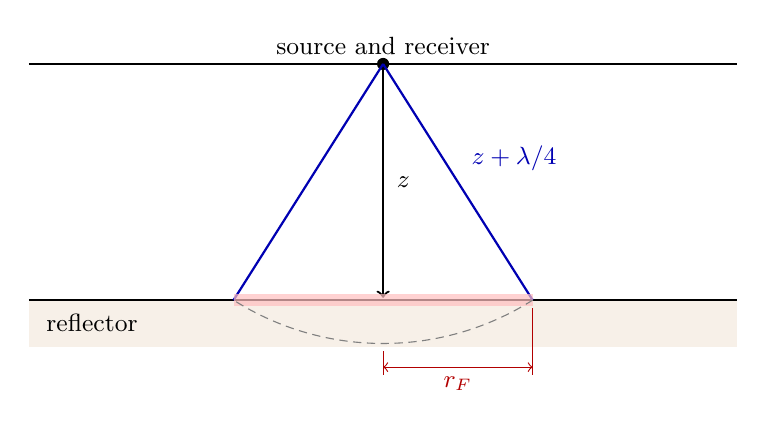
\begin{tikzpicture}[font=\small, x=1cm, y=1cm]
\fill[brown!12] (-4.5,-3.6) rectangle (4.5,-3.0);
\draw[thick] (-4.5,-3.0) -- (4.5,-3.0);
\node[anchor=north west] at (-4.4,-3.05) {reflector};
\draw[thick] (-4.5,0) -- (4.5,0);
\fill (0,0) circle (2.2pt) node[above] {source and receiver};
\draw[->, thick] (0,0) -- (0,-2.97);
\node[anchor=west] at (0.05,-1.5) {$z$};
\draw[blue!70!black, thick] (0,0) -- (1.9,-3.0);
\draw[blue!70!black, thick] (0,0) -- (-1.9,-3.0);
\node[anchor=west, blue!70!black] at (1.0,-1.2) {$z + \lambda/4$};
\fill[red!25, opacity=0.7] (-1.9,-3.08) rectangle (1.9,-2.92);
\draw[red!70!black] (0,-3.65) -- (0,-3.95) (1.9,-3.1) -- (1.9,-3.95);
\draw[<->, red!70!black] (0,-3.85) -- (1.9,-3.85) node[midway, below] {$r_F$};
\draw[gray, densely dashed] (-57.6:3.55) arc (-57.6:-122.4:3.55);
\end{tikzpicture}

\par\smallskip{\small The first \omterm{def:b3:exploration-seismology:fresnel}{Fresnel zone} (schematic): the part of the
reflector whose distance from a coincident source and receiver exceeds the
normal distance $z$ by less than $\lambda/4$ (dashed arc: the sphere of radius
$z + \lambda/4$), so that the two-way excess path is under half a wavelength
and its echoes arrive in phase. The scale of $\lambda$ is exaggerated.}
\label{fig:b3:exploration-seismology:fresnel}
\end{omfigure}

\section{Common-midpoint acquisition and processing}

A single echo is too faint to see in the noise. Reflection surveys therefore
record each subsurface point many times, with different source--receiver pairs,
and add the records.

\begin{definition}[Common midpoint, fold]\label{def:b3:exploration-seismology:cmp}
For a source at $x_s$ and a receiver at $x_r$ on a line, the midpoint is
$(x_s + x_r)/2$ and the offset $x = |x_r - x_s|$. A \emph{common
midpoint}\index{common midpoint} (CMP) gather is the set of traces, from all the
shots, that share the same midpoint; over flat layers they all reflect from the
same subsurface point. The \emph{fold (of seismic coverage)}\index{fold (of seismic coverage)}
is the number of traces in a gather. With $N$ channels at the
receiver interval $\Delta g$ and a shot every $\Delta s$ along the line, the fold
is $N\Delta g/(2\Delta s)$.
\end{definition}

\begin{omfigure}
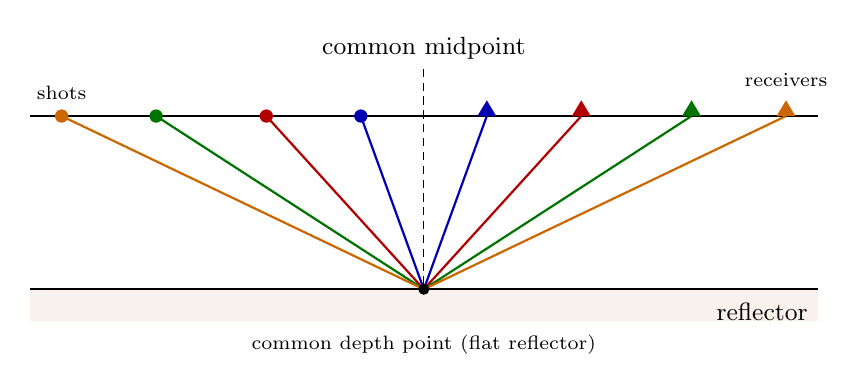
\begin{tikzpicture}[font=\small, x=1cm, y=1cm]
\draw[thick] (-5,0) -- (5,0);
\fill[brown!10] (-5,-2.6) rectangle (5,-2.2);
\draw[thick] (-5,-2.2) -- (5,-2.2);
\node[anchor=north east] at (5,-2.25) {reflector};
\foreach \off/\col in {0.8/blue!70!black, 2.0/red!70!black, 3.4/green!45!black, 4.6/orange!80!black} {
  \draw[\col, thick] (-\off,0) -- (0,-2.2) -- (\off,0);
  \fill[\col] (-\off,0) circle (2.4pt);
  \fill[\col] (\off-0.12,0) -- (\off+0.12,0) -- (\off,0.2) -- cycle;
}
\fill (0,-2.2) circle (2pt);
\draw[densely dashed] (0,0.6) -- (0,-2.2);
\node[anchor=south] at (0,0.6) {common midpoint};
\node[anchor=north, align=center, font=\scriptsize] at (0,-2.65) {common depth point (flat reflector)};
\node[anchor=south, font=\scriptsize] at (-4.6,0.08) {shots};
\node[anchor=south, font=\scriptsize] at (4.6,0.25) {receivers};
\end{tikzpicture}

\par\smallskip{\small Common-midpoint geometry (schematic): four source--receiver
pairs (dots, triangles) of different offsets share the same midpoint; over a
flat reflector they all reflect at the same point below it. Their traces form a
gather of fold four.}
\label{fig:b3:exploration-seismology:cmp}
\end{omfigure}

\begin{theorem}[Normal moveout]\label{thm:b3:exploration-seismology:nmo}
In a layer of speed $v$ over a flat reflector at the two-way vertical time
$t_0$, the reflection recorded at offset $x$ arrives at
\[
  t(x)^2 = t_0^2 + \frac{x^2}{v^2},
\]
a hyperbola in the $(x, t)$ plane. The delay $\Delta t = t(x) - t_0$ is the
\emph{normal moveout}\index{normal moveout}; for $x \ll vt_0$,
$\Delta t \approx x^2/(2v^2t_0)$.
\end{theorem}

\begin{proof}
The reflection path goes from the source to the reflection point under the
midpoint and back up to the receiver: two legs of length
$\sqrt{(vt_0/2)^2 + (x/2)^2}$. So $t = (2/v)\sqrt{(vt_0/2)^2 + (x/2)^2}$ and
$t^2 = t_0^2 + x^2/v^2$. Then $t - t_0 = (t^2 - t_0^2)/(t + t_0) \approx
x^2/(2v^2t_0)$.
\end{proof}

Over several layers the reflection time is no longer exactly hyperbolic, but it
is nearly so at small offsets, with a speed that is a weighted mean of the
layers'.

\begin{definition}[Stacking, root-mean-square and interval velocities]\label{def:b3:exploration-seismology:velocities}
The \emph{interval velocity}\index{interval velocity} $v_i$ of a layer is its
own speed; with $\Delta t_i = 2h_i/v_i$ the two-way time across it, the
\emph{root-mean-square velocity}\index{root-mean-square velocity} down to the
base of layer $n$ is
\[
  V_{\text{rms},n} = \left(\frac{\sum_{i\le n}v_i^2\,\Delta t_i}{\sum_{i\le n}\Delta t_i}\right)^{1/2}.
\]
The \emph{stacking velocity}\index{stacking velocity} of a reflection is the
speed $V$ of the hyperbola $t^2 = t_0^2 + x^2/V^2$ that best fits its times in a
CMP gather.
\end{definition}

\begin{proposition}[Stacking velocity at small offsets]\label{prop:b3:exploration-seismology:rms}
Over flat layers, $t(x)^2 = t_0^2 + x^2/V_{\text{rms}}^2 + O(x^4)$: at small
offsets, the \omterm{def:b3:exploration-seismology:velocities}{stacking velocity} is the RMS velocity.
\end{proposition}

\begin{proof}
For the \omterm{def:b3:seismology-imaging:ray-parameter}{ray parameter} $p$, $x = \sum_i 2h_i\tan\varphi_i$ and
$t = \sum_i 2h_i/(v_i\cos\varphi_i)$, with $\sin\varphi_i = pv_i$. To second
order in $p$, $\tan\varphi_i \approx pv_i$ and $1/\cos\varphi_i \approx 1 +
p^2v_i^2/2$, so $x \approx p\sum v_i^2\Delta t_i = pV_{\text{rms}}^2t_0$ and
$t \approx t_0 + \tfrac12p^2V_{\text{rms}}^2t_0$. Then
$t^2 \approx t_0^2 + p^2V_{\text{rms}}^2t_0^2 = t_0^2 + x^2/V_{\text{rms}}^2$, the
neglected terms being of order $p^4$, that is $x^4$.
\end{proof}

\begin{theorem}[Dix equation]\label{thm:b3:exploration-seismology:dix}
If $V_{n-1}$ and $V_n$ are the RMS velocities to the top and the base of layer
$n$, at the two-way times $t_{n-1}$ and $t_n$, the \omterm{def:b3:exploration-seismology:velocities}{interval velocity} of the
layer is given by the \emph{Dix equation}\index{Dix equation}
\[
  v_n^2 = \frac{V_n^2t_n - V_{n-1}^2t_{n-1}}{t_n - t_{n-1}} ,
\]
and its thickness is $h_n = v_n(t_n - t_{n-1})/2$.
\end{theorem}

\begin{proof}
By definition $V_n^2t_n = \sum_{i\le n}v_i^2\Delta t_i$ and $V_{n-1}^2t_{n-1}
= \sum_{i\le n-1}v_i^2\Delta t_i$. Their difference is $v_n^2\Delta t_n$, with
$\Delta t_n = t_n - t_{n-1}$.
\end{proof}

Velocity analysis scans each gather for the hyperbola that best fits the
energy: for each trial $t_0$ and $V$, the traces are summed along the curve, and
a coherence measure (the semblance) is mapped; the analyst picks its maxima,
reflector by reflector, to build a velocity function. The NMO correction then
shifts every sample of every trace from $t(x)$ to $t_0$, flattening the
reflections, and the traces of each gather are added.

\begin{definition}[Stacking (seismic)]\label{def:b3:exploration-seismology:stack}
\emph{Stacking (seismic)}\index{stacking (seismic)} is the summation, after the
normal-moveout correction, of the traces of a CMP gather into a single trace
placed at the midpoint. The stacked traces, side by side along the line, form
the stacked section, an image of the reflectors in two-way time.
\end{definition}

\begin{proposition}[Gain of a stack]\label{prop:b3:exploration-seismology:sqrtN}
If the $N$ traces of a gather carry the same reflection signal and independent
noise of equal standard deviation $\sigma$, their mean carries the same signal
and noise of standard deviation $\sigma/\sqrt N$: stacking raises the
signal-to-noise ratio by $\sqrt N$.
\end{proposition}

\begin{proof}
The variance of a sum of $N$ independent variables is the sum of their
variances, $N\sigma^2$; divided by $N^2$, the mean has the variance
$\sigma^2/N$ (the standard deviation of the mean, recalled from the
mathematics books).
\end{proof}

\begin{omfigure}
\begin{tikzpicture}
\begin{groupplot}[group style={group size=2 by 1, horizontal sep=0.5cm, y descriptions at=edge left},
  width=0.52\linewidth, height=0.56\linewidth, y dir=reverse, ymin=0.4, ymax=0.92,
  xmin=-150, xmax=2150, tick label style={font=\scriptsize}, title style={font=\small},
  xlabel={\scriptsize offset (\unit{m})}]
\nextgroupplot[title={(a) CMP gather}, ylabel={two-way time (\unit{s})}]
\addplot[black, very thin, unbounded coords=jump] table[x=x, y=t] {figdata/out/bachelor-3-cmp_nmo-gather-raw.dat};
\nextgroupplot[title={(b) after NMO correction}]
\addplot[black, very thin, unbounded coords=jump] table[x=x, y=t] {figdata/out/bachelor-3-cmp_nmo-gather-nmo.dat};
\end{groupplot}
\end{tikzpicture}

\par\smallskip{\small A synthetic CMP gather beneath the syncline axis of the
Varden line (computed by exact ray tracing through the flat-layered column; 30
Hz \omterm{def:b3:exploration-seismology:wavelet}{Ricker wavelet}; no noise). (a) The four reflections (top of the shale, top
and base of the limestone, top of the basement) curve down with offset along
near-hyperbolae. (b) After the NMO correction with the stacking velocities
fitted on the offsets up to \qty{600}{m}, the reflections are flat out to about
\qty{1}{km}; beyond, the true times depart from the hyperbola and the
correction leaves them bent, and the wavelets are stretched; in processing,
the stretched far traces of the shallow reflections are muted before the
stack.}
\label{fig:b3:exploration-seismology:gather}
\end{omfigure}

\begin{omfigure}
\begin{tikzpicture}
\begin{axis}[omrecord, width=0.72\linewidth, height=0.46\linewidth,
  xmin=0.4, xmax=0.78, ymin=2000, ymax=5000,
  xlabel={two-way time $t_0$ (\unit{s})}, ylabel={velocity (\unit{m.s^{-1}})},
  legend cell align=left, legend columns=2,
  legend style={font=\scriptsize, at={(0.5,-0.24)}, anchor=north}]
\addplot[gray, thick, const plot mark right] table[x=t0, y=vint] {figdata/out/bachelor-3-cmp_nmo-vel.dat};
\addlegendentry{interval velocity of the model}
\addplot[gray, thick, forget plot] coordinates {(0.4,2500) (0.487847,2500)};
\addplot[blue!70!black, thick, mark=*, mark size=1.5pt] table[x=t0, y=vrms] {figdata/out/bachelor-3-cmp_nmo-vel.dat};
\addlegendentry{RMS velocity}
\addplot[red!70!black, only marks, mark=square*, mark size=1.6pt] table[x=t0, y=vstack] {figdata/out/bachelor-3-cmp_nmo-vel.dat};
\addlegendentry{stacking velocity (offsets to \qty{600}{m})}
\addplot[green!45!black, only marks, mark=triangle*, mark size=2pt] table[x=t0, y=vdix] {figdata/out/bachelor-3-cmp_nmo-vel.dat};
\addlegendentry{Dix interval velocity}
\end{axis}
\end{tikzpicture}

\par\smallskip{\small Velocities beneath the syncline axis (computed). The RMS
velocity, a weighted mean, changes slowly; the stacking velocities of the
gather lie close to it. Applied to them, the \omterm{thm:b3:exploration-seismology:dix}{Dix equation} recovers the \omterm{def:b3:exploration-seismology:velocities}{interval
velocity} of each layer (the step line, drawn at the base of each layer) to
within a few per cent, the error growing in the thin, fast limestone.}
\label{fig:b3:exploration-seismology:velocities}
\end{omfigure}

\begin{omfigure}
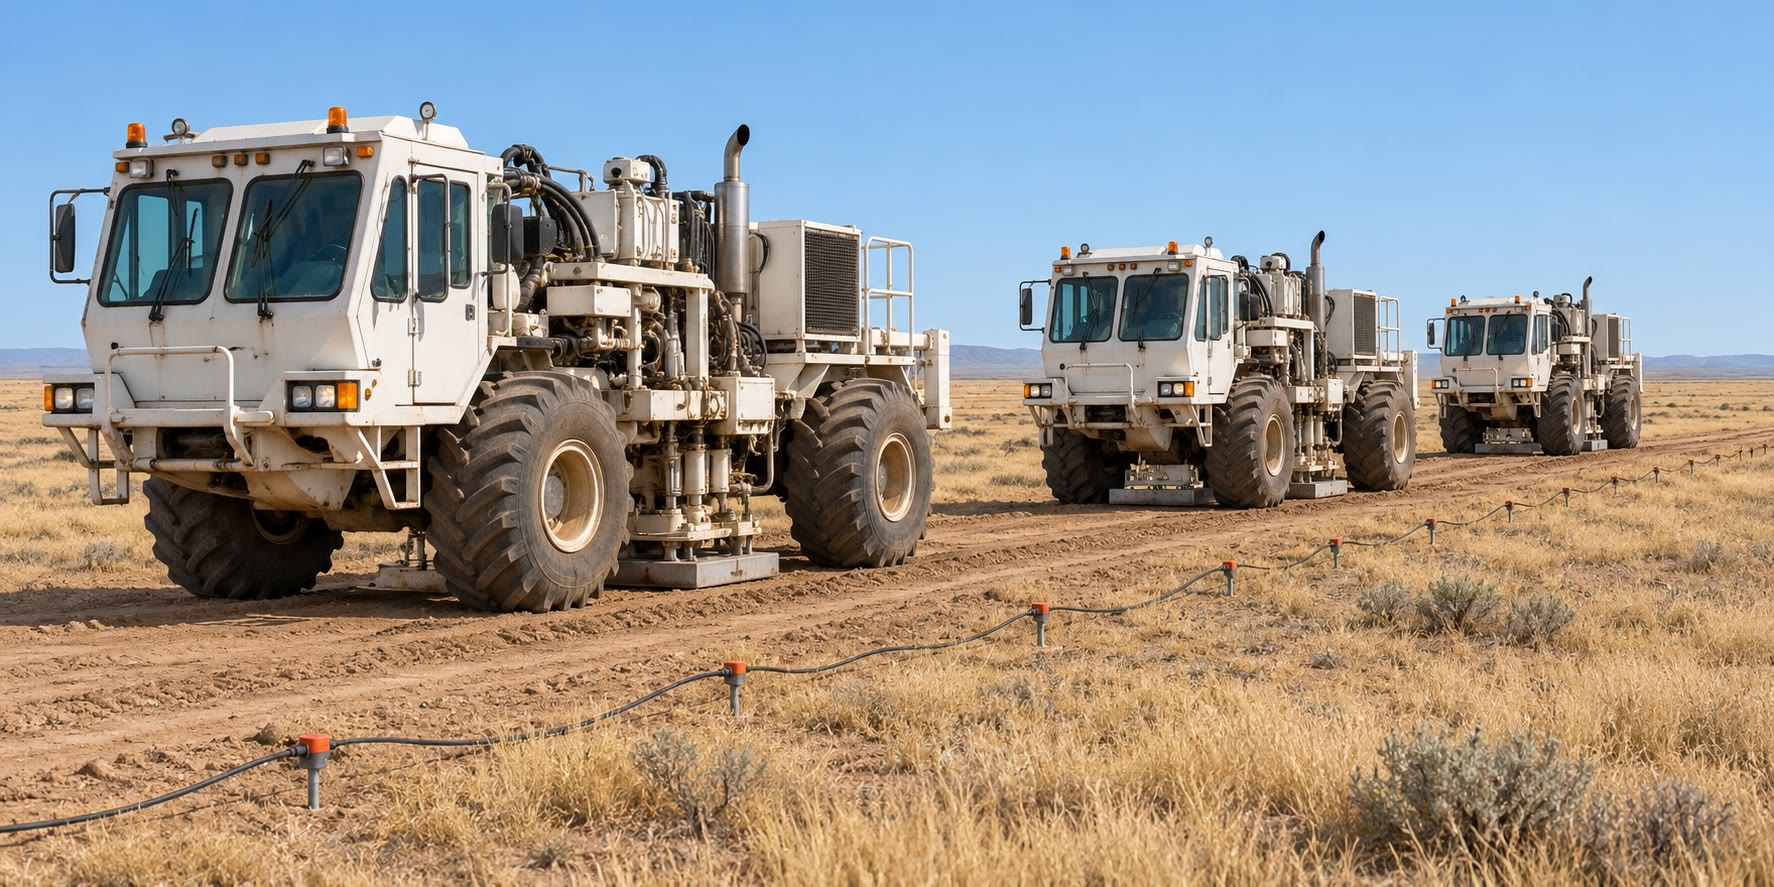
\includegraphics[width=0.62\linewidth]{images/book5/ai/b3-vibroseis.jpg}

\par\smallskip{\small Vibrator trucks on a land survey line: instead of an
explosion, each truck presses a heavy plate on the ground and shakes it with a
sweep of frequencies for several seconds; the long records are compressed into
short pulses by correlating them with the sweep (AI-generated illustration).}
\label{fig:b3:exploration-seismology:vibroseis}
\end{omfigure}

\section{Migration}

A stacked section shows each reflection under the midpoint where it was
recorded, at the time it took to come back. For a flat reflector that is where
it is. For a dipping one it is not: the echo recorded at a surface point comes
from the point of the reflector nearest to it, which lies up-dip, not
vertically below. Points such as fault cut-offs, which scatter energy in all
directions, appear as hyperbolae.

\begin{definition}[Seismic migration]\label{def:b3:exploration-seismology:migration}
\emph{Seismic migration}\index{seismic migration} is the processing step that
moves the reflections of a seismic section to the positions of the reflectors
that produced them: it restores the true dips and positions of dipping
reflectors and collapses the diffraction hyperbolae of point scatterers onto
their apices. Done with a velocity model in time, it gives a time-migrated
section; with a model in depth, a depth image.
\end{definition}

\begin{theorem}[Dip on a zero-offset section]\label{thm:b3:exploration-seismology:dip}
In a medium of speed $v$, a plane reflector of dip $\theta$ in the plane of the
section appears on the zero-offset section, plotted as the depth $vt/2$
vertically below each recording point, as a line of apparent dip $\theta_a$
with
\[
  \tan\theta_a = \sin\theta .
\]
The reflection recorded at the point $x$ comes from the reflector point a
distance $(vt/2)\sin\theta$ up-dip of the point vertically below $x$.
\end{theorem}

\begin{proof}
The zero-offset ray is normal to the reflector, so the time recorded at $x$ is
$t = 2d(x)/v$, where $d(x)$ is the distance from $x$ to the plane. That distance
grows by $\sin\theta$ for each unit of $x$ in the dip direction, so the plotted
depth $vt/2 = d(x)$ has the slope $\sin\theta$. The foot of the normal from $x$
to the plane lies at the horizontal distance $d\sin\theta$ from $x$, on the
up-dip side.
\end{proof}

Since $\tan\theta_a = \sin\theta < \tan\theta$, an unmigrated section always
shows dips gentler than the true ones, and it cannot show dips steeper than
\ang{45} at all. A point scatterer at depth $z$ below the point $x_0$ returns at
$x$ the zero-offset time $t(x) = (2/v)\sqrt{z^2 + (x - x_0)^2}$: a hyperbola with
its apex over the point, the diffraction. Migration in its simplest form,
the diffraction stack, sums each section along the diffraction hyperbola of
every possible scatterer and puts the sum at the apex: reflectors, which are
continuous lines of scatterers, emerge in their true places, and the
diffractions collapse.

\begin{omfigure}
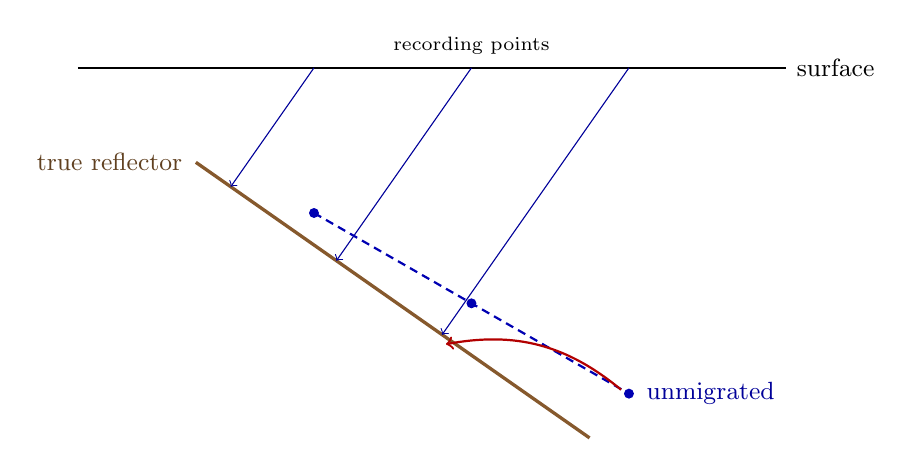
\begin{tikzpicture}[font=\small, x=1cm, y=1cm]
\draw[thick] (-0.5,0) -- (8.5,0) node[right] {surface};
% true reflector, dip 35 deg, rising to the left
\draw[very thick, brown!70!black] (1.0,-1.2) -- (6.0,-4.70);
\node[brown!50!black, anchor=east] at (0.95,-1.2) {true reflector};
% zero-offset normal rays from x = 2, 4, 6
\foreach \x in {2.5, 4.5, 6.5} {
  % distance from (x,0) to the line through (1,-1.2) dir (cos35,-sin35): normal n=(sin35,cos35)
  \pgfmathsetmacro{\dd}{abs(0.5736*(\x-1.0) + 0.8192*(0+1.2))}
  \draw[blue!60!black, ->] (\x,0) -- ++({-0.5736*\dd},{-0.8192*\dd});
  \fill[blue!70!black] (\x,{-\dd}) circle (1.8pt);
}
% apparent reflector through the plotted points
\pgfmathsetmacro{\da}{abs(0.5736*1.5 + 0.8192*1.2)}
\pgfmathsetmacro{\db}{abs(0.5736*5.5 + 0.8192*1.2)}
\draw[blue!70!black, thick, densely dashed] (2.5,{-\da}) -- (6.5,{-\db});
\node[blue!60!black, anchor=west] at (6.6,{-\db}) {unmigrated};
\node[anchor=south, font=\scriptsize] at (4.5,0.05) {recording points};
\draw[->, red!70!black, thick] (6.4,{-\db+0.05}) to[bend right=25] ({6.5-0.5736*\db+0.05},{-0.8192*\db-0.12});
\end{tikzpicture}

\par\smallskip{\small Migration of a dipping reflector (schematic, true dip
\ang{35}). The zero-offset ray at each recording point is normal to the
reflector, so its echo comes from up-dip; plotted vertically below the point,
at the depth $vt/2$, the reflection appears gentler (dashed: $\tan\theta_a =
\sin\theta$, here \ang{29.8}), and displaced down-dip. Migration (red arrow) moves it back.}
\label{fig:b3:exploration-seismology:migration}
\end{omfigure}

\section{Seismic stratigraphy}

A migrated section is a picture of the layering, and it can be read as
stratigraphy: the reflections follow the bedding surfaces, which are
time lines, so their geometry records how the basin filled.

\begin{definition}[Seismic stratigraphy, seismic facies]\label{def:b3:exploration-seismology:seismic-stratigraphy}
\emph{Seismic stratigraphy}\index{seismic stratigraphy} is the interpretation
of the stratigraphy and depositional history of a basin from the geometry of
its seismic reflections. A \emph{seismic facies}\index{seismic facies} is a
three-dimensional unit of reflections whose character (continuity, amplitude,
frequency, internal geometry: parallel, divergent, sigmoid, chaotic, mounded)
differs from that of its neighbours and is interpreted as a depositional
environment.
\end{definition}

\begin{definition}[Reflection terminations]\label{def:b3:exploration-seismology:terminations}
A \emph{reflection termination}\index{reflection termination} is the end of a
reflection against another. \emph{Onlap}\index{onlap}: an initially horizontal
reflection ends against a surface that rises more steeply, the younger beds
lapping onto an older slope. \emph{Downlap}\index{downlap}: an inclined
reflection ends down-dip against a gentler surface, as the toes of prograding
beds rest on the floor of a basin. \emph{Toplap}\index{toplap}: inclined
reflections end up-dip against an overlying surface, with little erosion, as
the tops of prograding beds meet the level of the sea. \emph{Erosional
truncation}\index{erosional truncation}: reflections end up-dip against an
overlying surface that cuts them, an unconformity.
\end{definition}

\begin{omfigure}
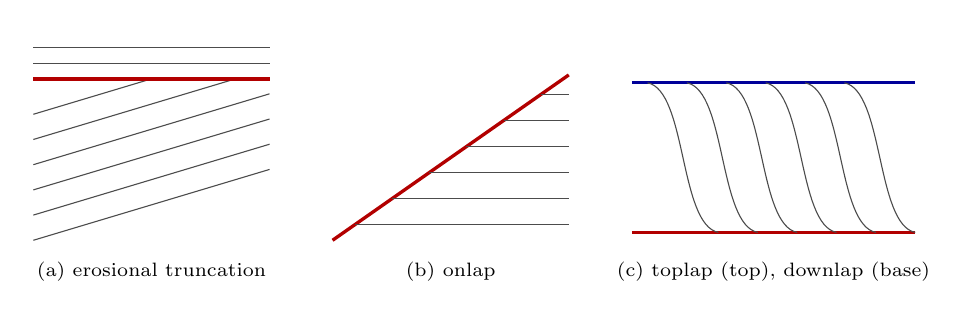
\begin{tikzpicture}[font=\scriptsize, x=1cm, y=1cm]
% erosional truncation: tilted beds cut by an unconformity
\begin{scope}
\foreach \k in {0,...,5} {\draw[gray!60!black] (0,{-2.3+0.32*\k}) -- (3.0,{-1.4+0.32*\k-0.25*0});}
\fill[white] (0,-0.25) -- (3.2,-0.25) -- (3.2,0.4) -- (0,0.4) -- cycle;
\draw[very thick, red!70!black] (0,-0.25) -- (3.0,-0.25);
\foreach \k in {0,1} {\draw[gray!60!black] (0,{-0.05+0.2*\k}) -- (3.0,{-0.05+0.2*\k});}
\node[anchor=north] at (1.5,-2.45) {(a) erosional truncation};
\end{scope}
% onlap
\begin{scope}[xshift=3.8cm]
\draw[very thick, red!70!black] (0,-2.3) -- (3.0,-0.2);
\foreach \k in {0,...,5} {\pgfmathsetmacro{\y}{-2.1+0.33*\k} \pgfmathsetmacro{\xe}{(\y+2.3)/0.7} \draw[gray!60!black] (\xe,\y) -- (3.0,\y);}
\node[anchor=north] at (1.5,-2.45) {(b) onlap};
\end{scope}
% downlap and toplap: clinoforms
\begin{scope}[xshift=7.6cm]
\draw[very thick, red!70!black] (0,-2.2) -- (3.6,-2.2);
\draw[very thick, blue!60!black] (0,-0.3) -- (3.6,-0.3);
\foreach \k in {0,...,5} {\draw[gray!60!black] ({0.2+0.5*\k},-0.3) .. controls ({0.7+0.5*\k},-0.4) and ({0.6+0.5*\k},-2.1) .. ({1.1+0.5*\k},-2.2);}
\node[anchor=north] at (1.8,-2.45) {(c) toplap (top), downlap (base)};
\end{scope}
\end{tikzpicture}

\par\smallskip{\small \omterm{def:b3:exploration-seismology:terminations}{Reflection terminations} (schematic sections, grey
reflections, terminating surfaces in colour). (a) Tilted reflections cut by an
unconformity. (b) Flat reflections ending against an older slope. (c) Inclined
beds of a prograding wedge ending up-dip against the surface above (\omterm{def:b3:exploration-seismology:terminations}{toplap}) and
down-dip on the basin floor (\omterm{def:b3:exploration-seismology:terminations}{downlap}).}
\label{fig:b3:exploration-seismology:terminations}
\end{omfigure}

The terminations mark the surfaces that bound sequences of genetically related
beds; mapping them across a basin, and relating them to the rise and fall of
relative sea level, is sequence stratigraphy, the subject of
\cref{ch:b3:sequence-stratigraphy}. A seismic section of a passive margin
typically shows wedges of seaward-prograding reflections downlapping onto the
deep floor, capped by \omterm{def:b3:exploration-seismology:terminations}{toplap}, and buried landward under onlapping beds laid
down when the sea rose again.

\begin{inthefield}[A marine streamer survey and a land crew]
\begin{minipage}[t]{0.55\linewidth}\vspace{0pt}
On a marine survey the vessel never stops: it sails line after line at a few
knots, the air-gun arrays firing at fixed intervals, the streamers held at a
constant depth by small steerable wings and located by acoustic and satellite
positioning. Observers on the bridge watch the sea around the array, and the
survey works under rules that set out the measures to protect marine mammals,
the watch kept and what is reported.
% ledger: noaa5:itr-gom
On land the crew lays out cables or wireless recording units along the lines;
vibrator trucks advance in convoy from one source point to the next, and a
recording truck checks every channel before each sweep. Back in the processing
centre the records are sorted into common-midpoint gathers, the velocities
picked, the data stacked and migrated, and the section handed to the
interpreters.
\end{minipage}\hfill
\begin{minipage}[t]{0.42\linewidth}\vspace{0pt}
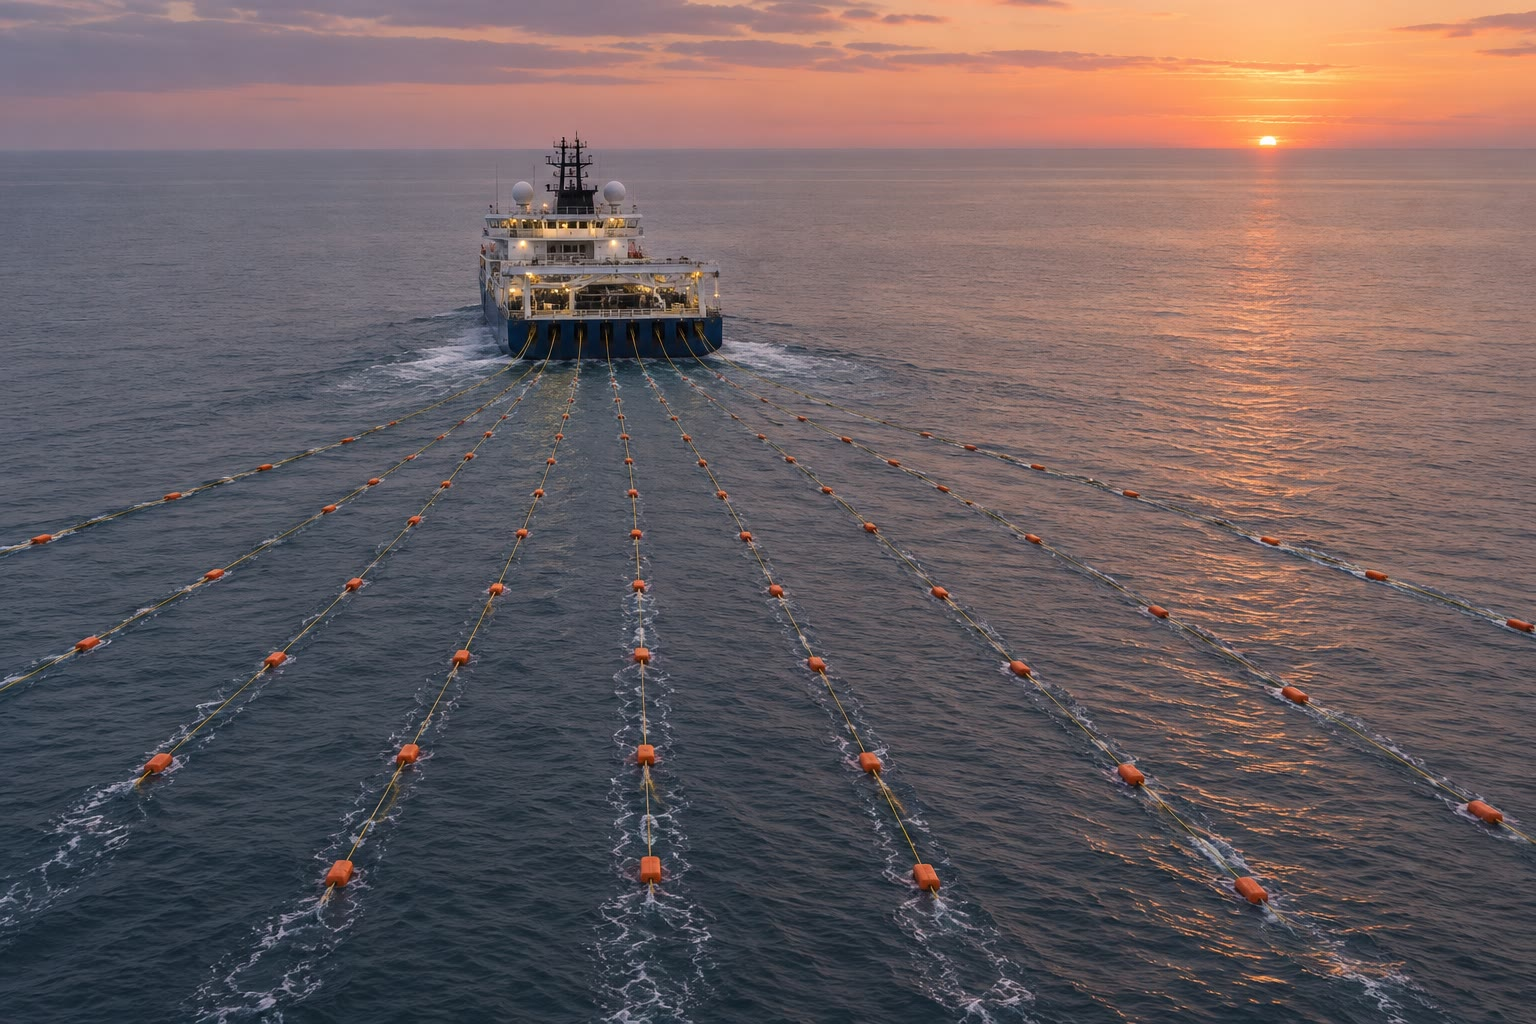
\includegraphics[width=\linewidth]{images/book5/ai/b3-streamer-vessel.jpg}

{\scriptsize A seismic survey vessel towing its streamers at dusk
(AI-generated illustration).}
\end{minipage}
\end{inthefield}

\section{Exercises}

\begin{exercise}[$\star$]\label{exo:b3:exploration-seismology:1}
Chalk ($v = \qty{2500}{m.s^{-1}}$, $\rho = \qty{2.00}{g.cm^{-3}}$) lies on shale
(\qty{2300}{m.s^{-1}}, \qty{2.30}{g.cm^{-3}}), which lies on limestone
(\qty{4500}{m.s^{-1}}, \qty{2.60}{g.cm^{-3}}). Compute the three impedances and
the reflection coefficients of the two interfaces. What fraction of the incident
energy does the top of the limestone reflect?
% ledger: mavko:velocities
\end{exercise}

\begin{exercise}[$\star$]\label{exo:b3:exploration-seismology:2}
A flat reflector lies \qty{800}{m} below a layer of \qty{2000}{m.s^{-1}}.
Compute $t_0$, the reflection time at an offset of \qty{1000}{m}, and the \omterm{thm:b3:exploration-seismology:nmo}{normal
moveout} there. Compare with the approximation $x^2/(2v^2t_0)$.
\end{exercise}

\begin{exercise}[$\star$]\label{exo:b3:exploration-seismology:3}
A streamer has 240 channels \qty{12.5}{m} apart, and the vessel fires every
\qty{25}{m}. Compute the CMP interval and the fold. What shot interval would
give a fold of 120?
\end{exercise}

\begin{exercise}[$\star$]\label{exo:b3:exploration-seismology:4}
With a dominant frequency of \qty{30}{Hz}, compute the wavelength and the
quarter wavelength in sandstone of \qty{3000}{m.s^{-1}} and in limestone of
\qty{4500}{m.s^{-1}}. Compute the radius of the first \omterm{def:b3:exploration-seismology:fresnel}{Fresnel zone} of a
reflector \qty{1000}{m} deep under rocks of mean speed \qty{2800}{m.s^{-1}}.
\end{exercise}

\begin{exercise}[$\star\star$]\label{exo:b3:exploration-seismology:5}
Two reflections have $t_0 = \qty{0.500}{s}$ with an RMS velocity of
\qty{2400}{m.s^{-1}}, and $t_0 = \qty{0.700}{s}$ with \qty{2800}{m.s^{-1}}.
Compute the \omterm{def:b3:exploration-seismology:velocities}{interval velocity} and the thickness of the layer between them.
\end{exercise}

\begin{exercise}[$\star\star$]\label{exo:b3:exploration-seismology:6}
A plane reflector dips at $\varphi$ in the plane of a CMP line, in a layer of
speed $v$. (a) Show that $t(x)^2 = t_0^2 + x^2\cos^2\varphi/v^2$, where $t_0$ is
the zero-offset time at the midpoint. (Hint: use the image of the midpoint in
the reflector.) (b) Deduce the \omterm{def:b3:exploration-seismology:velocities}{stacking velocity}, and compute it for
$v = \qty{2000}{m.s^{-1}}$ and $\varphi = \ang{12}$.
\end{exercise}

\begin{exercise}[$\star\star$]\label{exo:b3:exploration-seismology:7}
A gather of fold 60 has independent noise of equal variance on every trace. By
what factor does stacking raise the signal-to-noise ratio? By what factor must
the fold be increased to double it again?
\end{exercise}

\begin{exercise}[$\star\star$]\label{exo:b3:exploration-seismology:8}
On a zero-offset time section, in rock of \qty{3000}{m.s^{-1}}, a reflection
rises by \qty{0.40}{s} of two-way time per kilometre along the line. Convert this
slope into an apparent dip, and compute the true dip of the reflector.
\end{exercise}

\begin{exercise}[$\star\star$]\label{exo:b3:exploration-seismology:9}
Convolve the \omterm{def:b3:exploration-seismology:synthetic}{reflectivity series} $r = (0, 0.3, 0, -0.2, 0)$ with the
three-sample wavelet $w = (-0.5, 1, -0.5)$, sample by sample. Where are the two
reflections, and do they overlap?
\end{exercise}

\begin{exercise}[$\star\star\star$]\label{exo:b3:exploration-seismology:10}
A reversed refraction profile over a layer of \qty{1800}{m.s^{-1}} gives a
down-dip apparent velocity of \qty{2900}{m.s^{-1}} and an up-dip one of
\qty{4400}{m.s^{-1}}. Compute the critical angle, the dip and the refractor
speed. Compare the refractor speed with the harmonic mean of the two apparent
speeds.
\end{exercise}

\begin{exercise}[$\star\star\star$]\label{exo:b3:exploration-seismology:11}
In \cref{prop:b3:exploration-seismology:tuning}, a bed has reflection
coefficients $+R$ and $-R$. (a) Show that for $\Delta t \ll T$ the composite
signal is approximately $R\,\Delta t\,w'(t)$, the time derivative of the wavelet
scaled by the bed's two-way thickness. (b) Explain why a thin bed can still be
detected, though not resolved, and how its thickness could be estimated from
its amplitude. (c) Two beds of the same rock, 5 and \qty{10}{m} thick, are
imaged with the same wavelet: what is the ratio of their amplitudes?
\end{exercise}

\begin{exercise}[$\star\star\star$]\label{exo:b3:exploration-seismology:12}
A point scatterer lies \qty{600}{m} below the line, in rock of
\qty{3000}{m.s^{-1}}. (a) Write the zero-offset time of its diffraction against
the horizontal distance $x$ from the point above it, and compute it at $x = 0$
and \qty{300}{m}. (b) Show that the diffraction is a hyperbola of the NMO form
with the speed $v/2$, and explain why a diffraction is always more curved than a
reflection with the same apex time. (c) What does migration do to it?
\end{exercise}

\section{Problem: A Seismic Line across the Varden Hills}

\begin{problem}[{Weekend problem --- refraction, velocity analysis, depth
conversion and migration along section A--B of the Varden Hills}]
\label{pb:b3:exploration-seismology:1}
% values: calc/ch02.py, from figdata seismic_model.py, refraction_dip.py, cmp_nmo.py
A seismic line is shot along section A--B of the Varden Hills, the region of
the geological maps of the earlier volumes. Its distances $s$ are counted from
A along the line. The cover, from the top, is chalk, shale (\qty{100}{m}),
limestone (\qty{180}{m}) and sandstone (\qty{120}{m}), resting unconformably on
a schist basement; it is folded into an anticline and a syncline and cut by a
normal fault.

\medskip
\noindent\textbf{Part I --- A refraction spread on the west limb.} A spread of
\qty{1200}{m} is laid between shot points W ($s = \qty{300}{m}$) and E
($s = \qty{1500}{m}$), on ground taken as level. The chalk and shale above the
limestone are treated as one layer of $v_1 = \qty{2.40}{km.s^{-1}}$. The
head-wave times read on the records are, from W towards E, \qty{425.2}{ms} at
\qty{800}{m} and \qty{486.1}{ms} at \qty{1200}{m}; from E towards W,
\qty{372.4}{ms} at \qty{800}{m} and \qty{486.1}{ms} at \qty{1200}{m}.
\begin{enumerate}
  \item Compute the two apparent speeds. Which shot is up-dip?
  \item Compute the critical angle and the dip of the refractor.
  \item Compute the speed of the refractor. Which rock is it?
  \item Compute the intercept times and the perpendicular depths of the
        refractor under W and under E.
  \item Convert them to vertical depths, and check the dip from the two depths.
  \item The shale under the chalk is slower than the chalk. What does the
        refraction survey make of it, and how does it bias the depths?
\end{enumerate}

\noindent\textbf{Part II --- Velocity analysis at CMP S.} Further east, CMP S
lies on the axis of the syncline, in the downthrown block of the fault, where
the layers are taken as flat. Four reflections are picked at zero offset and at
\qty{600}{m}:
\begin{center}
\small
\begin{tabular}{lcccc}
\hline
reflection & 1 & 2 & 3 & 4 \\
$t_0$ (\unit{s}) & 0.4878 & 0.5748 & 0.6548 & 0.7348 \\
$t(\qty{600}{m})$ (\unit{s}) & 0.5437 & 0.6240 & 0.6887 & 0.7648 \\
\hline
\end{tabular}
\end{center}
\begin{enumerate}[resume]
  \item Compute the NMO velocity $V = x/\sqrt{t^2 - t_0^2}$ of reflections 1
        and 2. Why is the second smaller than the first?
  \item Compute it for reflections 3 and 4.
  \item Taking these as RMS velocities, compute the \omterm{def:b3:exploration-seismology:velocities}{interval velocity} of each
        layer by the \omterm{thm:b3:exploration-seismology:dix}{Dix equation}.
  \item Identify the layers from their speeds, and name the four reflecting
        interfaces.
  \item Reflection 1 is the faintest on the records. Why?
  \item Why were the velocities measured on the offsets up to \qty{600}{m}
        only, when the spread reaches \qty{2}{km}?
\end{enumerate}

\noindent\textbf{Part III --- Depth conversion and resolution.}
\begin{enumerate}[resume]
  \item Compute the two-way time spent in each layer and its thickness.
  \item Compute the depth of each reflecting interface below the ground. Compare
        the thicknesses of the shale, limestone and sandstone with the values
        given above.
  \item Compute the mean speed from the ground to the basement, and explain why
        the NMO velocity of reflection 4 would overestimate the depth if used
        instead.
  \item The survey's wavelet peaks at \qty{30}{Hz}. Compute the wavelength in
        the shale and its \omterm{def:b3:exploration-seismology:resolution}{tuning thickness}, both by the quarter-wavelength rule
        and by $b = v/(5.2f)$ for a \omterm{def:b3:exploration-seismology:wavelet}{Ricker wavelet}. Is the shale resolved? At
        what frequency would it tune by the quarter-wavelength rule?
  \item Compute the radius of the first \omterm{def:b3:exploration-seismology:fresnel}{Fresnel zone} on the basement, taking
        $\lambda$ from the NMO velocity of reflection 4.
\end{enumerate}

\noindent\textbf{Part IV --- Migration and the fault.}
\begin{enumerate}[resume]
  \item Near the fault, the cut-off of the limestone produces a diffraction
        whose apex is at \qty{0.550}{s}; \qty{200}{m} from the apex along the line
        it is at \qty{0.5732}{s}. Write the zero-offset diffraction time and
        deduce the mean speed above the cut-off.
  \item Compute the depth of the cut-off below the ground.
  \item On the east limb, the top-limestone reflection of the stacked section
        rises towards the anticline by \qty{0.167}{s} of two-way time per
        kilometre, under rocks of mean speed \qty{2.48}{km.s^{-1}}. Compute its
        apparent dip and its true dip.
  \item A reflection on that limb is recorded at $t = \qty{0.655}{s}$. How far,
        and in which direction, does migration move it?
  \item Across the fault the top-basement reflection jumps by \qty{0.160}{s};
        the downthrown block carries the extra thickness in chalk. Compute the
        throw.
  \item Give the depth of the basement unconformity below CMP S, from the
        interval velocities of Part II.
\end{enumerate}
\end{problem}
